\documentclass{article}
\usepackage{etoolbox}
\usepackage{graphicx}

\ifdef{\myoutput}{}{\def\myoutput{concept}}
\ifdef{\myversion}{}{\def\myversion{1}}

\usepackage[output=\myoutput
,numberofversions=4
,version=\myversion
,seed=4
,randomizequestions=true
,randomizeanswers=true
,writeRfile=true
]{mcexam}

\usepackage[margin=0.95in]{geometry}
\usepackage{multicol}

\usepackage{fancyhdr,lastpage}
\pagestyle{fancy}
\fancyhf{}
\renewcommand{\headrulewidth}{1pt} 
\renewcommand{\footrulewidth}{1pt}
\lfoot{\mctheversion}
\rfoot{Page \thepage\ of \pageref{LastPage}}
\lhead{Quiz 3.2 Version \fbox{\myversion} \\ MAT 2000: Introduction to Statistics}
\rhead{Name Print): \hspace{2.5 in}}

\usepackage{calc}
\renewenvironment{setmcquestion}
{\begin{minipage}[t]{\linewidth-\labelwidth}}
	{\end{minipage}\par}
	
\renewenvironment{setmcquestioninstruction}
{\begin{minipage}{\textwidth}}
	{\end{minipage}}
	
\renewenvironment{setmcanswers}{}{}
\setlist[setmcquestions]{label=\mcquestionlabelfmt{*}.
	,ref=\mcquestionlabelfmt{*}
	,itemsep=0.5\baselineskip
	,topsep=1\baselineskip
}

\renewcommand\mcversionlabelfmt[1]{\arabic{#1}}

%\mcifoutput{exam}{
%	\AtEndDocument{\ifodd\value{page}
%		\newpage\thispagestyle{empty}\hbox{This page intentionally left blank.}\newpage\thispagestyle{empty}\hbox{}
%		\else
%		\newpage\thispagestyle{empty}\hbox{}
%		\fi}
%}

\raggedbottom

\begin{document}
	Circle the correct answer for each question.  If you're unsure, you can write numbers 1, 2, 3, etc. next to the choices to get partial credit.\\[.5cm]
	\begin{mcquestions}
		\begin{mcquestioninstruction}
			The following histogram shows the distribution of the difference between the actual and "ideal" weights for 119 female students. Ideal weights are responses to the question "What is your ideal weight"? The difference = actual – ideal.
			\begin{center}
				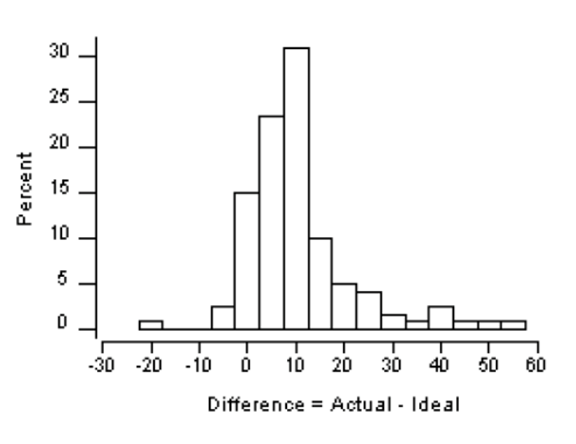
\includegraphics{ideal_weight.png}
			\end{center}
		\end{mcquestioninstruction}
				
		\question What is the approximate shape of the distribution?
		
		\begin{mcanswerslist}
			\answer[correct] The mean is larger than the median.
			\answer The median is larger than the mean.
			\answer The median and mean are approximately equal.
			\answer The mean and the median cannot be compared without calculations.			
		\end{mcanswerslist}
		
		\question[follow] How does the mean compare to the median in this data set?
		\begin{mcanswerslist}
			\answer[correct] The mean is larger than the median.
			\answer The median is larger than the mean.
			\answer The median and mean are approximately equal.
			\answer The mean and the median cannot be compared without calculations.
		\end{mcanswerslist}
		
		
		\question[follow] If the observation at -20 pounds was removed from the data set, the mean \_\_\_\_\_.
		
		\begin{mcanswerslist}
			\answer[correct] would increase
			\answer would decrease
			\answer would remain the same
			\answer may or may not change			
		\end{mcanswerslist}
		
		\begin{mcquestioninstruction}
			A hot dog manufacturer asserts that a brand of hot dogs has an average fat content of 18 grams per hot dog. Fat contents in hot dogs from this manufacturer follow an approximately normal distribution with a standard deviation of 1.1 grams. Define the statistic x = mean fat content in a random sample of 10 hot dogs.
		\end{mcquestioninstruction}
	
		\question The value 18 is the \_\_\_\_\_.
		\begin{mcanswerslist}
			\answer sample size
			\answer[correct] statistic
			\answer parameter
			\answer standard deviation
		\end{mcanswerslist}
		
		\question[follow] Is the sampling distribution of x approximately normal?
		\begin{mcanswerslist}
			\answer No, since the sample size is too small for the Central Limit Theorem to hold.
			\answer No, since the manufacturer does not know if the population of hot dogs is more than 20 times the size of the sample.
			\answer[correct] Yes, since the population of fat contents in hot dogs is approximately normal.
			\answer Not enough information exists to determine if the sampling distribution of x is approximately normal.
		\end{mcanswerslist}
		
		\question Which of the following distributions would have the smallest standard deviation?
		\begin{mcanswerslist}
			\answer Number of miles put on a rental car in one day
			\answer Average number of miles put on a rental car per day across 5 customers
			\answer[correct] Average number of miles put on a rental car per day across 25 customers
			\answer Distributions of all of the above would have the same standard deviation.
		\end{mcanswerslist}
		
	\end{mcquestions}
\end{document}